\documentclass[a4paper,11pt]{article}
\usepackage[T1]{fontenc}
\usepackage[utf8]{inputenc}
\usepackage{lmodern}
\usepackage{hyperref}
\usepackage{amsmath}
\usepackage{amssymb}
\usepackage{graphicx}

\title{Parallel Solution of Laplace's Equation}
\author{Leo Unbekandt}

\begin{document}

\maketitle
\tableofcontents

\begin{abstract}
  The main goal of this work is to develop a parallel way to solve numerically Laplace's Equation by using OpenMPI,
  and to analyze how this process accelerates the computation compare to the serial way to do, and how exact are the
  results compare to the analytical solution. The using method in this project must have been Jacobi with red-black
  ordering. However there is no interest in doing red-black ordering with Jacobi as we have to keep the old matrix in
  memory, that's why I've decided to use Gauss Seidel method associated with red-black ordering.
  
  The complete source code of this project may be found on Github: \url{https://github.com/Soulou/HPC_Assignment}
  It includes the analytical, the serial and the parallel methods, and additionaly the \LaTeX \hspace{5pt} source code of this
  report.
\end{abstract}

\section{The analytical solution}
\subsection{Solving the equation by using Fourier series}

Finding the analytical solution basically consists in solving:

$$\frac{\partial^2 \phi}{\partial y^2} + \frac{\partial^2 \phi}{\partial x^2} = 0 \hspace{2em} x \in [0,1], y \in [0,1]$$
The homogeneous boundary conditions are: 
$$\phi(x,0) = 0 \hspace{3em} \phi(x,1) = 0 \hspace{3em} \phi(1,y) = 0$$
The inhomogeneous boundary condition is: $$\phi(0,y) = sin^2(\pi y)$$
The separating the variables, we obtain $\phi(x,y) = X(x)Y(y)$, so Laplace's equation becomes:
$$\frac{1}{X}\frac{\partial^2 X}{\partial x^2} + \frac{1}{Y}\frac{\partial^2 Y}{\partial y^2} = 0$$
Let: $$\frac{1}{Y}\frac{\partial^2 Y}{\partial y^2} = - k^2 \Leftrightarrow Y(y) = A_1\cos(k y) + B_1\sin(k y)$$ 
So:
\begin{align*}
  \frac{1}{X}\frac{\partial^2 X}{\partial x^2} = k^2 \Leftrightarrow X(x) & = A_2\cosh(k x) + B_2\sinh(k x) \\
  Or: X(x) & = A_2\cosh(k (x-1)) + B_2\sinh(k (x-1))
\end{align*}
This second expression works better with $X(0) = 0$ as boundary condition. As a result we have:
$$\phi(x,y) = [ A_1\cos(k y) + B_1\sin(k y)][A_2\cosh(k (x-1)) + B_2\sinh(k (x-1))]$$
Thanks to our boundary conditions we deduce that
$$Y(0) = 0 \Rightarrow A_1=0 \hspace{2em} Y(1) = 0 \Rightarrow k=n \pi \hspace{2em} X(1) = 0 \Rightarrow A_2 = 0$$
Finally we get:
\begin{align*}
  \phi_n(x,y) & = B_n \sin(n \pi y)\sinh(n \pi (x-1)) & for\hspace{5pt}n \in \mathbb{N}^{+*} \\
  \phi_n(x,y) & = \sum_{n = 1}^{\infty}{B_n \sin(n \pi y)\sinh(n \pi (x-1))} & (by\hspace{5pt}superposition)
\end{align*}

Thanks to the inhomogeneous boundary condition we have:
\[
  \phi(0, y) = \sum_{n = 1}^{\infty}{B_n sin(n \pi y)\sinh(-n \pi)}
\]
The Fourier coefficient is now $B_n \sinh(-n \pi)$:
\begin{align*}
  B_n \sinh(-n \pi) & = \int_{0}^{1}{\sin^2(\pi y)\sin(n \pi y)dy} \\
  B_n & = \frac{2(\cos(\pi n) - 1)}{\pi(n^3 - 4n)\sinh(-n \pi)}
\end{align*}

\subsection{Implementation of the solution}
  The implementation has been done with the C programming language. The only constraint of using this language is
  that the result formula contains $\sinh(-n \pi)$. When $n$ gets bigger, a primitive variable type (double, long double)
  is not able anymore to have enough precision to compute correct results. This is why I've used the library
  GNU MPFR which is used to manipulate with high precision floating point numbers.
  
\subsection{Illustration of the analytical solution}

\begin{figure}[h!]
  \centering
  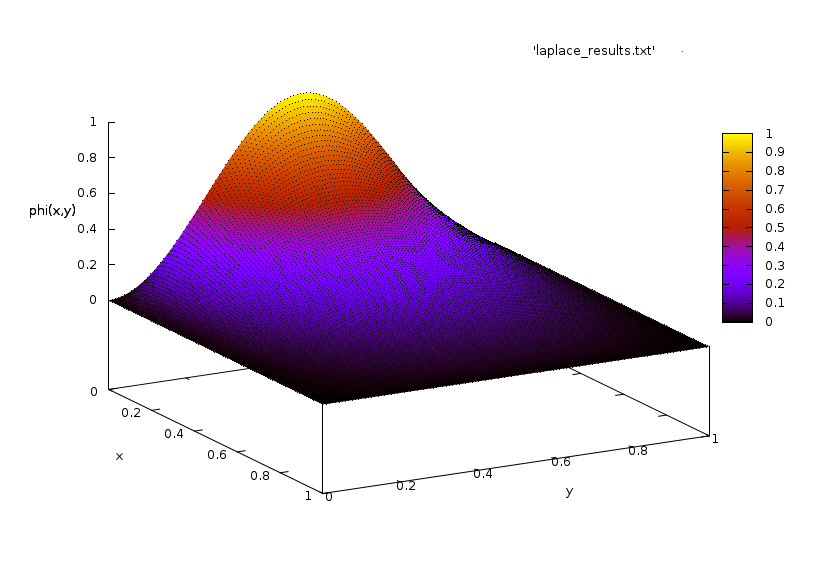
\includegraphics[width=0.8\textwidth]{images/analytical.png}
  \caption{Representation of $\phi(x,y)$ for a stepsize of 1/120}
\end{figure}

\section{The numerical solution - serial computation}
\subsection{Implementation}

\subsection{Aspect of the results}

\subsection{Validation of the implementation}

To know if the results are accurate we need to compare them to the results of the analytical solution. In order to
achieve that, I've developed a small script: \texttt{diff\_results.rb}. It compares two result files by calculating the
difference of each $\phi(x,y)$ and finally printing the average difference in percents. This difference represents the
average error of the numerical solution compare to the analytical one.

\section{OpenMPI - parallel computation}

\end{document}
